\documentclass[thesis.tex]{subfiles}

\begin{document}

\chapter{Prerequisites}\label{chap:preq}

This chapter lists and describes the necessary topics to follow this thesis. It explains SCION's structure, functionality and details about the component as for example the border router. SCIONLab itself and its work is also outlined. At last, a short description about Prometheus and its used features will be given.

\section{SCION}

SCION, an acronym for \textbf{S}calability, \textbf{C}ontrol and \textbf{I}solation \textbf{O}n \textbf{N}ext-generation networks, provides a green-field solution for problems of the current Internet. This is called in the content the \textit{legacy internet}. The main difference between them is \textit{path-transparency}. In the current existing IP routing protocol the end-hosts cannot chose a path, but must rely on the router between them to find a good path. This leads to the problem, that the receiver cannot verify, if the packets were modified nor if the taken path was trustworthy. SCION allows the end hosts to chose between communication paths and also to see the path of a packet on the end-host. The fundamental change needs a different organization of the network nodes, which will be described in this part.

\autoref{fig:prequirement:scionStructure} shows an example SCION network from \cite{SCIONPaper}. This topology consists of \textbf{Is}olation \textbf{D}omains (\textit{ISD}) and each node of it is considered an \textbf{A}utonomous \textbf{S}ystem (\textit{AS}). There is also a special group of ASes inside an ISD, the \textit{Core}. The Core Ases are responsible for connections between ISDs and can be seen as the ISD gateway. It is also possible to create a connection between two ASes of different ISDs without them as seen between AS C and the orange ISD.

When an AS wants to send data to another AS, it sends a \textit{path request} a \textit{path-server}, which can is normally located inside the ISDs Core. The respond contains a list of paths from the path-server to the requested target AS. This functionality leads not only to control over the path to take, but also to have alternatives. In the legacy internet a central node failure takes minutes to be resolved by the router,\todo{Quelle einfügen}, because the gateway router take some time to update their routing tables. With SCION an AS can choose another path, if existing, instead of waiting for an update.

One possibility originated from choosing a path is to send data via multiple path at the same time. 

\begin{figure}
	\centering
	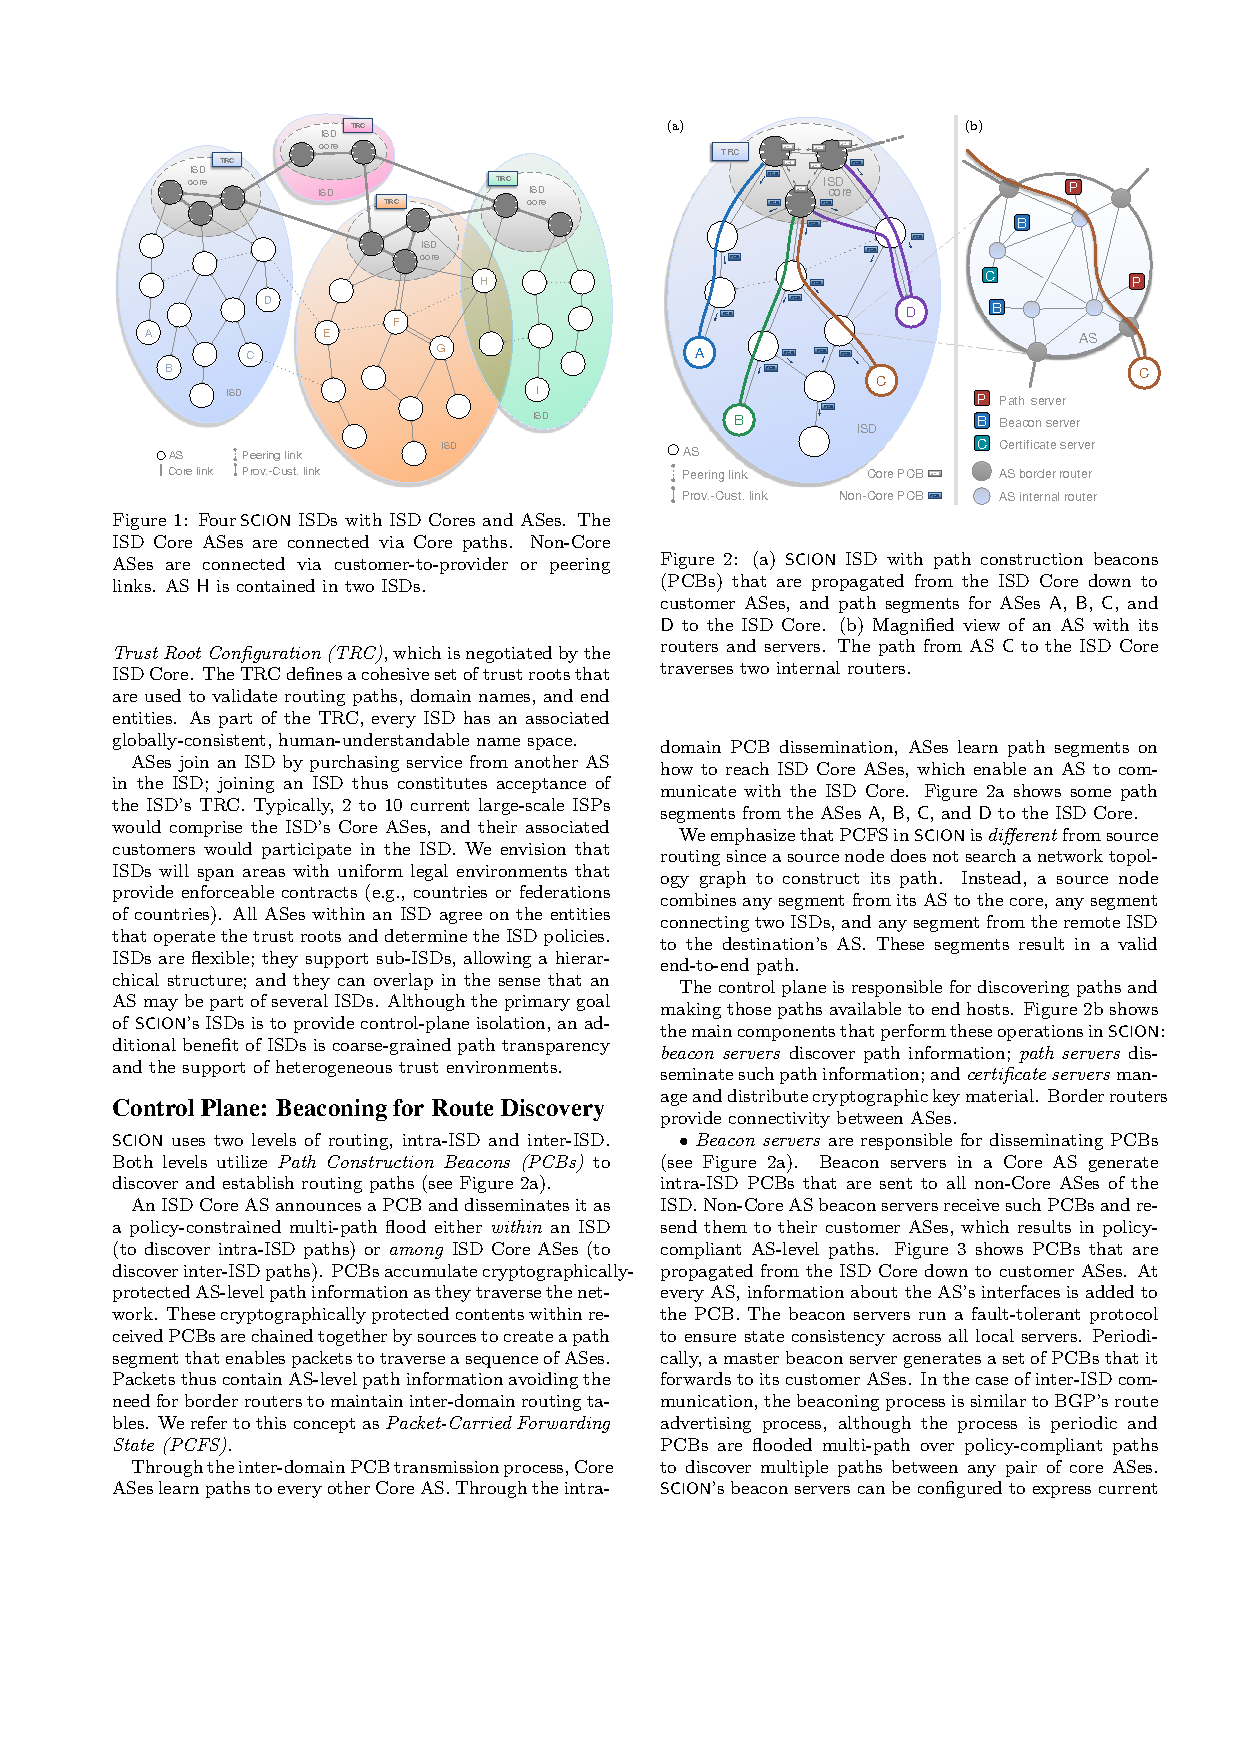
\includegraphics[trim=19mm 214mm 105mm 19mm ,clip,width=0.5\linewidth]{2015-SCION-short_3.pdf}
	\label{fig:prequirement:scionStructure}
	\caption{Four SCION ISDs with ISD Cores and ASes \cite{SCIONPaper}}
\end{figure}


\begin{easylist}
    \MyListProperties
    # SCION
    ## Origins of SCION
    ## Structure of SCION
    ## \textit{Figure example topology}
    ## Explain relevant components of an AS
    ### Path Server + Path Discovery
    ### Border Router
    ## SCIONLab
    ### Goal \& How it works
    ### Coordinator in ETH Zurich
    ## Multipath method
    ### How does it work
    ### \textit{Figure of example}
    ### Explanation of example
    ### Difference to legacy methods
    # Other prerequisites
\end{easylist}

\subfilebib % Makes bibliography available when compiling as subfile
\end{document}